\section{Electricity and Magnetism}
    \textbf{Electrical forces} occur between electric charges; \textbf{magnetic forces} occur between moving electric charges, or, electric currents. As a charge moves through space, it traces \textbf{electric and magnetic fields}, which are vector fields: vectors that have a value for every point in space. $\va{E}(\va{r})$ is electric field, and $\va{B}(\va{r})$. Electric charges are associated with electric fields and electric currents are associated with magnetic fields. The electric force is a conservative force and have a potential energy. By dividing out the charge that is feeling the electric field (test charge), we get something that only depends on the source charge distribution. This called \textbf{electric potential}.
    \begin{equation*}
        V(\va{r}) = - \int_{\va{r}_0}^{\va{r}}\va{E} \vdot d\va{r} + V(\va{r}_0)
    \end{equation*}
    Gauss' law is an equation that relates a field $F$ to its source $S$:
    \begin{equation*}
        \Phi_F = \iint \va{F} \vdot d\va{A} = \text{Constant} \vdot S
    \end{equation*}
    The most important fundamental laws of electricity and magnetism are known as the four \textbf{Maxwell's equations}.
    \subsection{Maxwell's Equations}
        \textbf{1. Gauss' law for electric fields}
            \begin{equation*}
                \Phi_E = \iint \va{E} \vdot d\va{A} = \frac{Q}{\epsilon_0}
            \end{equation*}
            where $Q$ is the net electric charge enclosed by the surface which he electric field is integrated. Gauss' law is equivalent to \textbf{Coulomb's Law} in static situations for the force between charges:
            \begin{equation*}
                \va{E} = \frac{q}{4\pi\epsilon_0r^2}\vu{r}
            \end{equation*}
            where $r$ is the distance from the point charge
            \newline
        \textbf{2. Gauss' law for magnetic fields}
            \begin{equation*}
                \Phi_B = \iint \va{B} \vdot d\va{A} = 0
            \end{equation*}
            This shows that there are no magnetic monopoles and the magnetic fields trace out closed loops instead of just pointing radially outwards.
            \newline
        \textbf{3. The generalized Ampere's law}
            \newline
            This relates magnetic fields to the currents and changing electric fields that produce them by the equation:
            \begin{equation*}
                \oint \va{B} \vdot d\va{s} = \mu_0I + \mu_0\epsilon_0\frac{d}{dt}\iint \va{E} \vdot d\va{A}
            \end{equation*}
            \begin{center}
                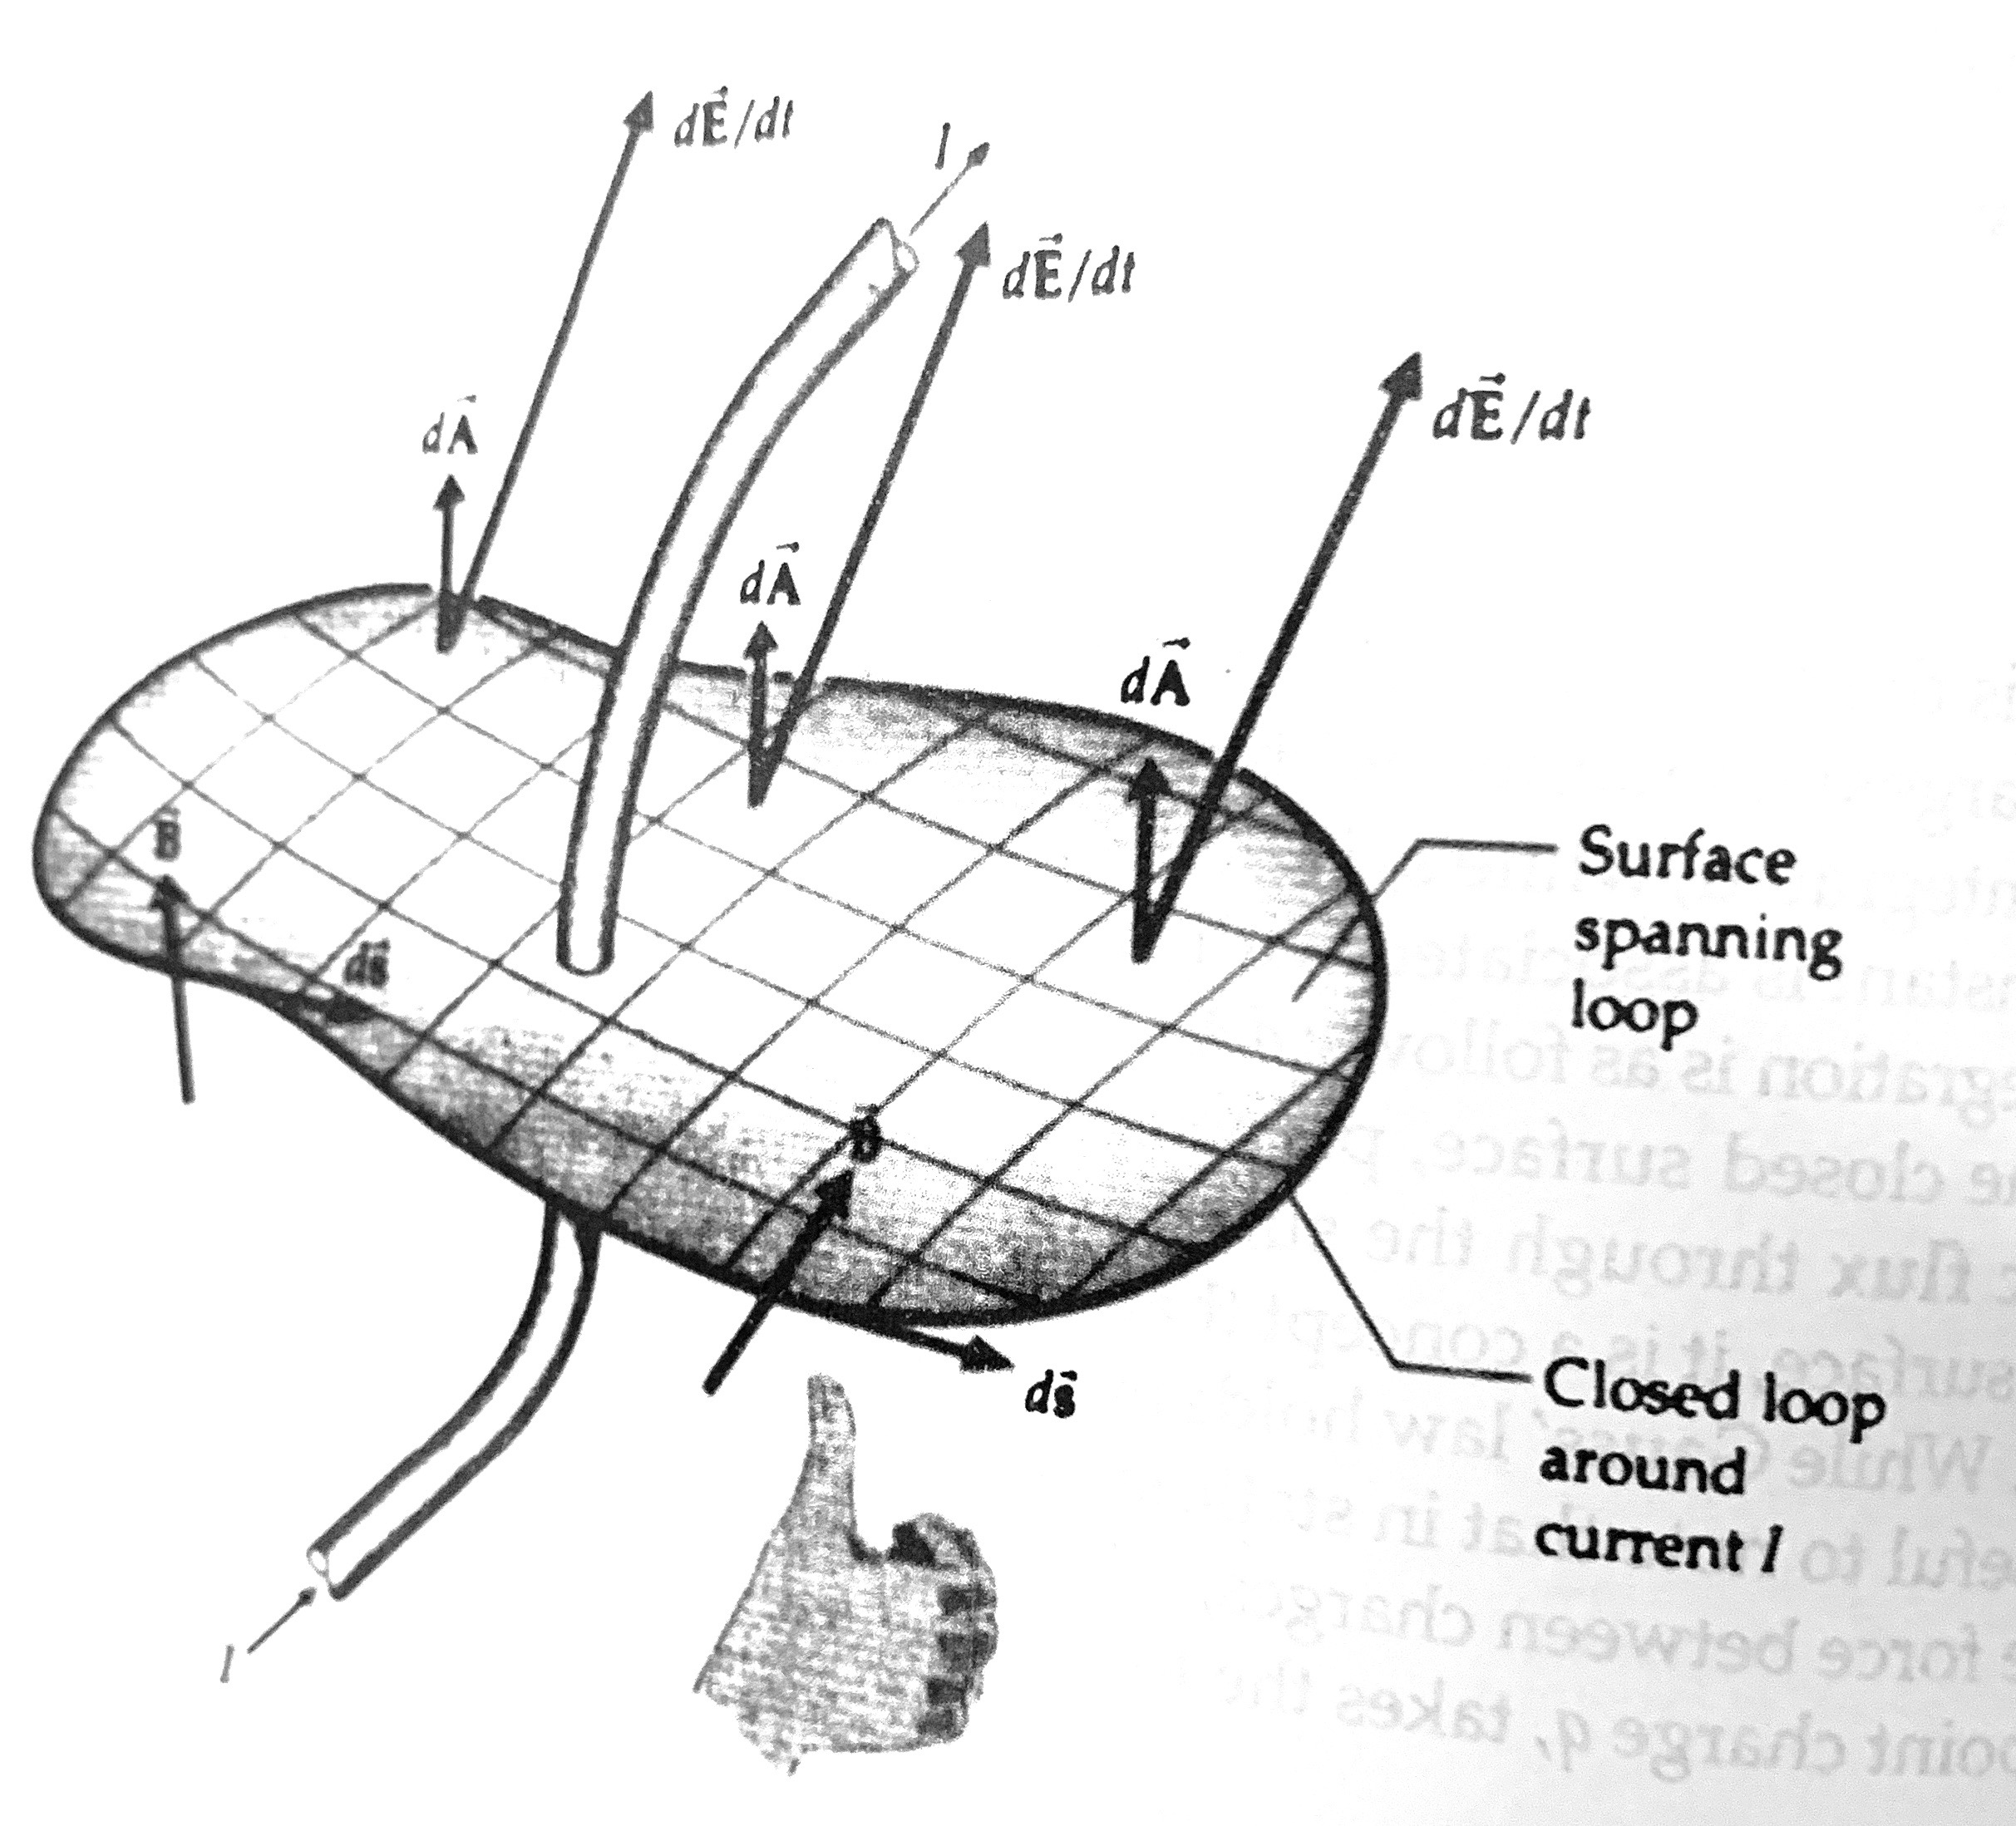
\includegraphics[width=200pt]{ampereslaw.jpg}
            \end{center}
            The double integral is the flux going through any surface that spans the loop. The first integral is a line integral around a closed loop enclosing the current $I$.
            \newline
        \textbf{4. Faraday's law:}
            \begin{equation*}
                \oint \va{E} \vdot d\va{s} = - \frac{d}{dt} \iint \va{B} \vdot d\va{A} 
            \end{equation*}
            Faraday's law demonstrates how changing magnetic flux can generate an electric field. The minus sign shows that the secondary / generated magnetic flux tends to oppose the original change in magnetic flux. This is known as \textbf{Lenz's law}.
            \newline
        \newline
        \newline
    \textbf{Lorentz force law}: the force on a charge $q$ moving with velocity $\va{v}$ in an electric field $\va{E}$ and magnetic field $\va{B}$
    \begin{equation*}
        \va{F} = q(\va{E} + \va{v} \cross \va{B})
    \end{equation*}
    so $\va{F} = \va{F}_E + \va{F}_B = q\va{E} + q(\va{v} \cross \va{B})$. $\va{F}_B$ can sometimes be written as a force on the length of a wire $d\va{\ell}$ carrying a current in a magnetic field.
    \begin{equation*}
        d\va{F}_B = I\va{\ell} \cross \va{B}
    \end{equation*}
    This can be integrated to find $\va{F}_B$.
    \newline \indent
    If a loop carrying current is placed in a uniform magnetic field $\va{B}$, theres no net force, but there is a torque that tends to twist the loop.
    \begin{equation*}
        \va{\tau} = \va{\mu} \cross \va{B}
    \end{equation*}
    where $\va{\mu}$ is the magnetic moment which is $I\va{A}$, where $I$ is the current carried in the loop and $\va{A}$ is the area of the loop with direction determined by the right hand rule (fingers following current and thumb at $\va{A}$). Torque tends to rotate the loop so that $\va{\mu}$ is in the same direction as $\va{B}$. When it is placed in the field, the loop has a minimum potential energy when $\va{\mu}$ and $\va{B}$ are aligned.
    \begin{equation*}
        U = - \va{\mu} \cross \va{B}
    \end{equation*}
    Electric and magnetic fields themselves contain energy. This is given by the energy density $u$, or energy per unit volume:
    \begin{equation*}
        u = \frac{1}{2\mu_0}B^2 + \frac{1}{2}\epsilon_0E^2
    \end{equation*}
    \textbf{Insulators} have the property that electric charges cannot move through them very easily. \textbf{Conductors} have the property that electrons can freely move within them. \textbf{Semiconductors} lie somewhere in between. 
    \newline \indent
    The  atoms of an insulator in an electric field align so that the electric field within the material is diminished. The effects of insulators, aka dielectrics, can be summarized by replacing $\epsilon_0$ with $\epsilon = \kappa\epsilon_0$, where $\kappa$ is the \textit{dielectric constant} of the material. The charges within conductors in an external electric field move until the electric field within is canceled. \textbf{Ferromagnetic} materials produce a magnetic field on their own by the alignment of its atoms which act like tiny magnets.
    \newline \indent
    \textit{Omn's law} descibes how currents in a piece of conducting material are formed when an electric field is maintained across the material.
    \begin{equation*}
        V = IR
    \end{equation*}
    where $V$ is the potential difference from end to end, $R$ is the resistance, and $I$ is the current. When $R$ is independent of $V$, the material is \textit{omnic} and Ohm's law applies.